\section{Performance}

The response of the LTCC to pions has been studied using experimental data containing ``good'' pion tracks.
The event selection is described below.

\subsection{Pions Selection}

Positive pion candidates $t$s are elected among positvely charged particles using the reaction $eP\rightArror e\pi^+N$. T
he criterias for event selections are:

\begin{itemize}
	\item Electrons identified using the reconstruction event builder algorithm;
    \item Electrons must be between 15\mdeg\ and 25\mdeg\ in $\theta$;
    \item Positive track candidates $t$s  identified using the reconstruction event builder algorithm;
    \item Positive track candidates must be between 10\mdeg\ and 25\mdeg\ in $\theta$ and between 94\mdeg\ and 108\mdeg\ in $\phi$;
	\item The neutron missing mass $e^-t^+(n)$ is applied between 0.9 and 1.05 GeV (see \F{neutronMM}).
\end{itemize}



\begin{figure}
	\centering
	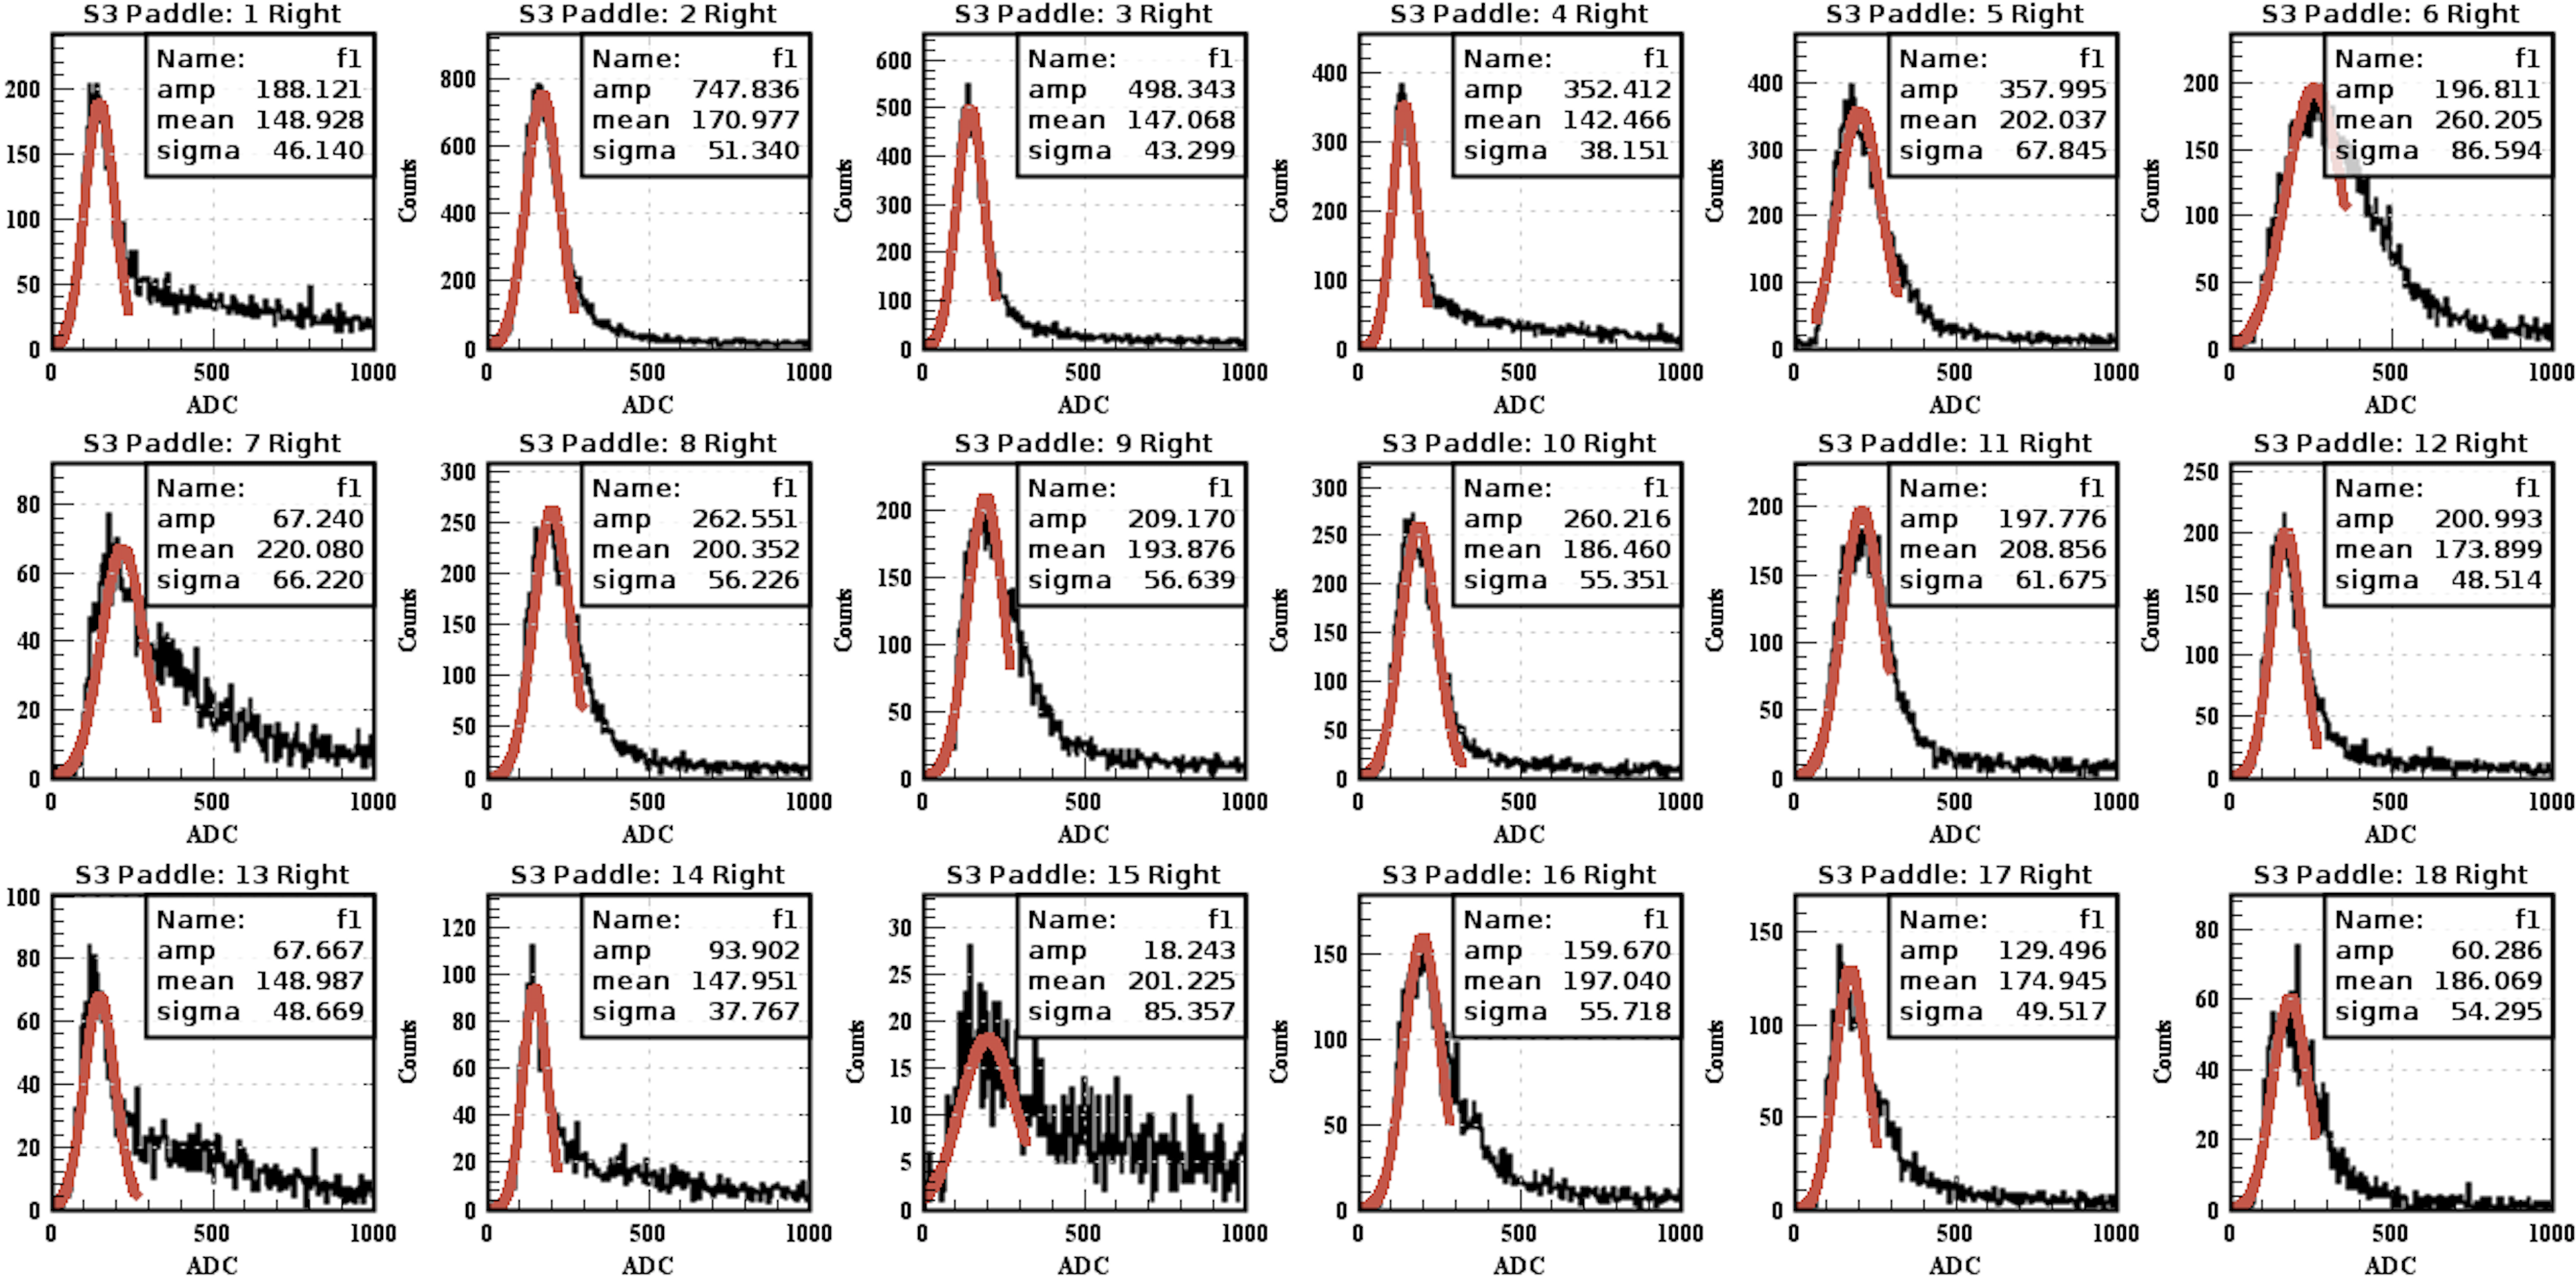
\includegraphics[width=0.98\columnwidth,keepaspectratio]{img/neutronMM.png}
	\caption{The neutron missing mass $e^-t^+(n)$.  }
	\label{fig:neutronMM}
\end{figure}






\subsection{LTCC Pions Response}

2 d plots of number of photoelectrons for both positive and negative pions


\begin{figure}
	\centering
	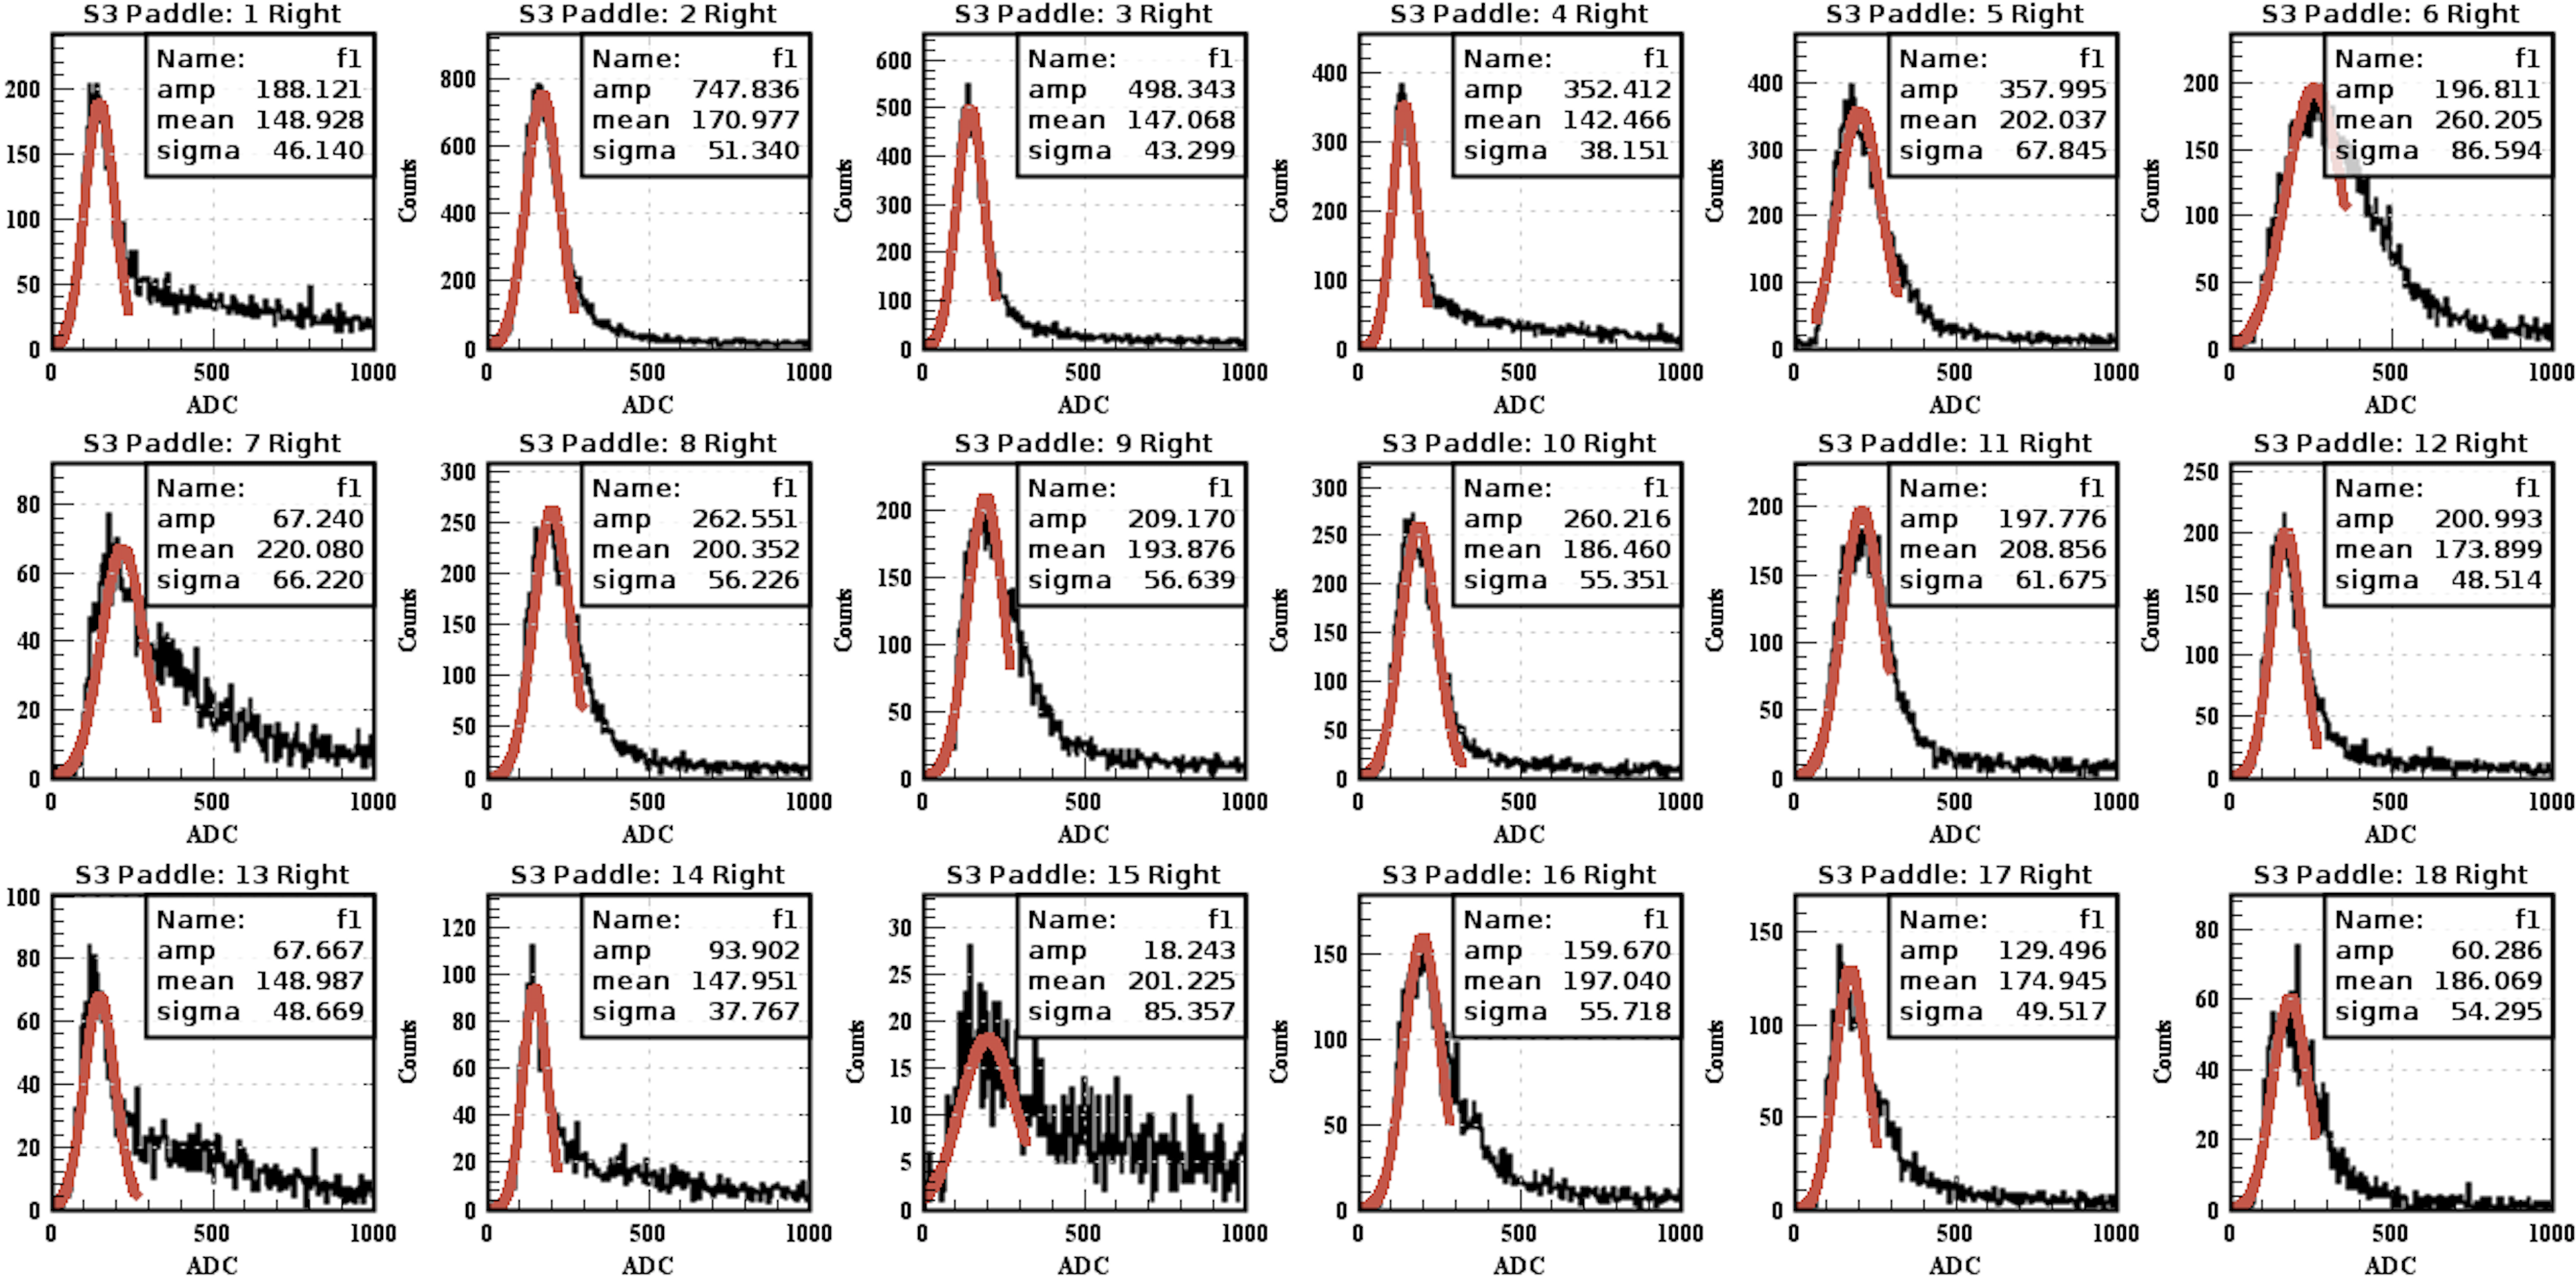
\includegraphics[width=0.98\columnwidth,keepaspectratio]{img/pipnphe.png}
	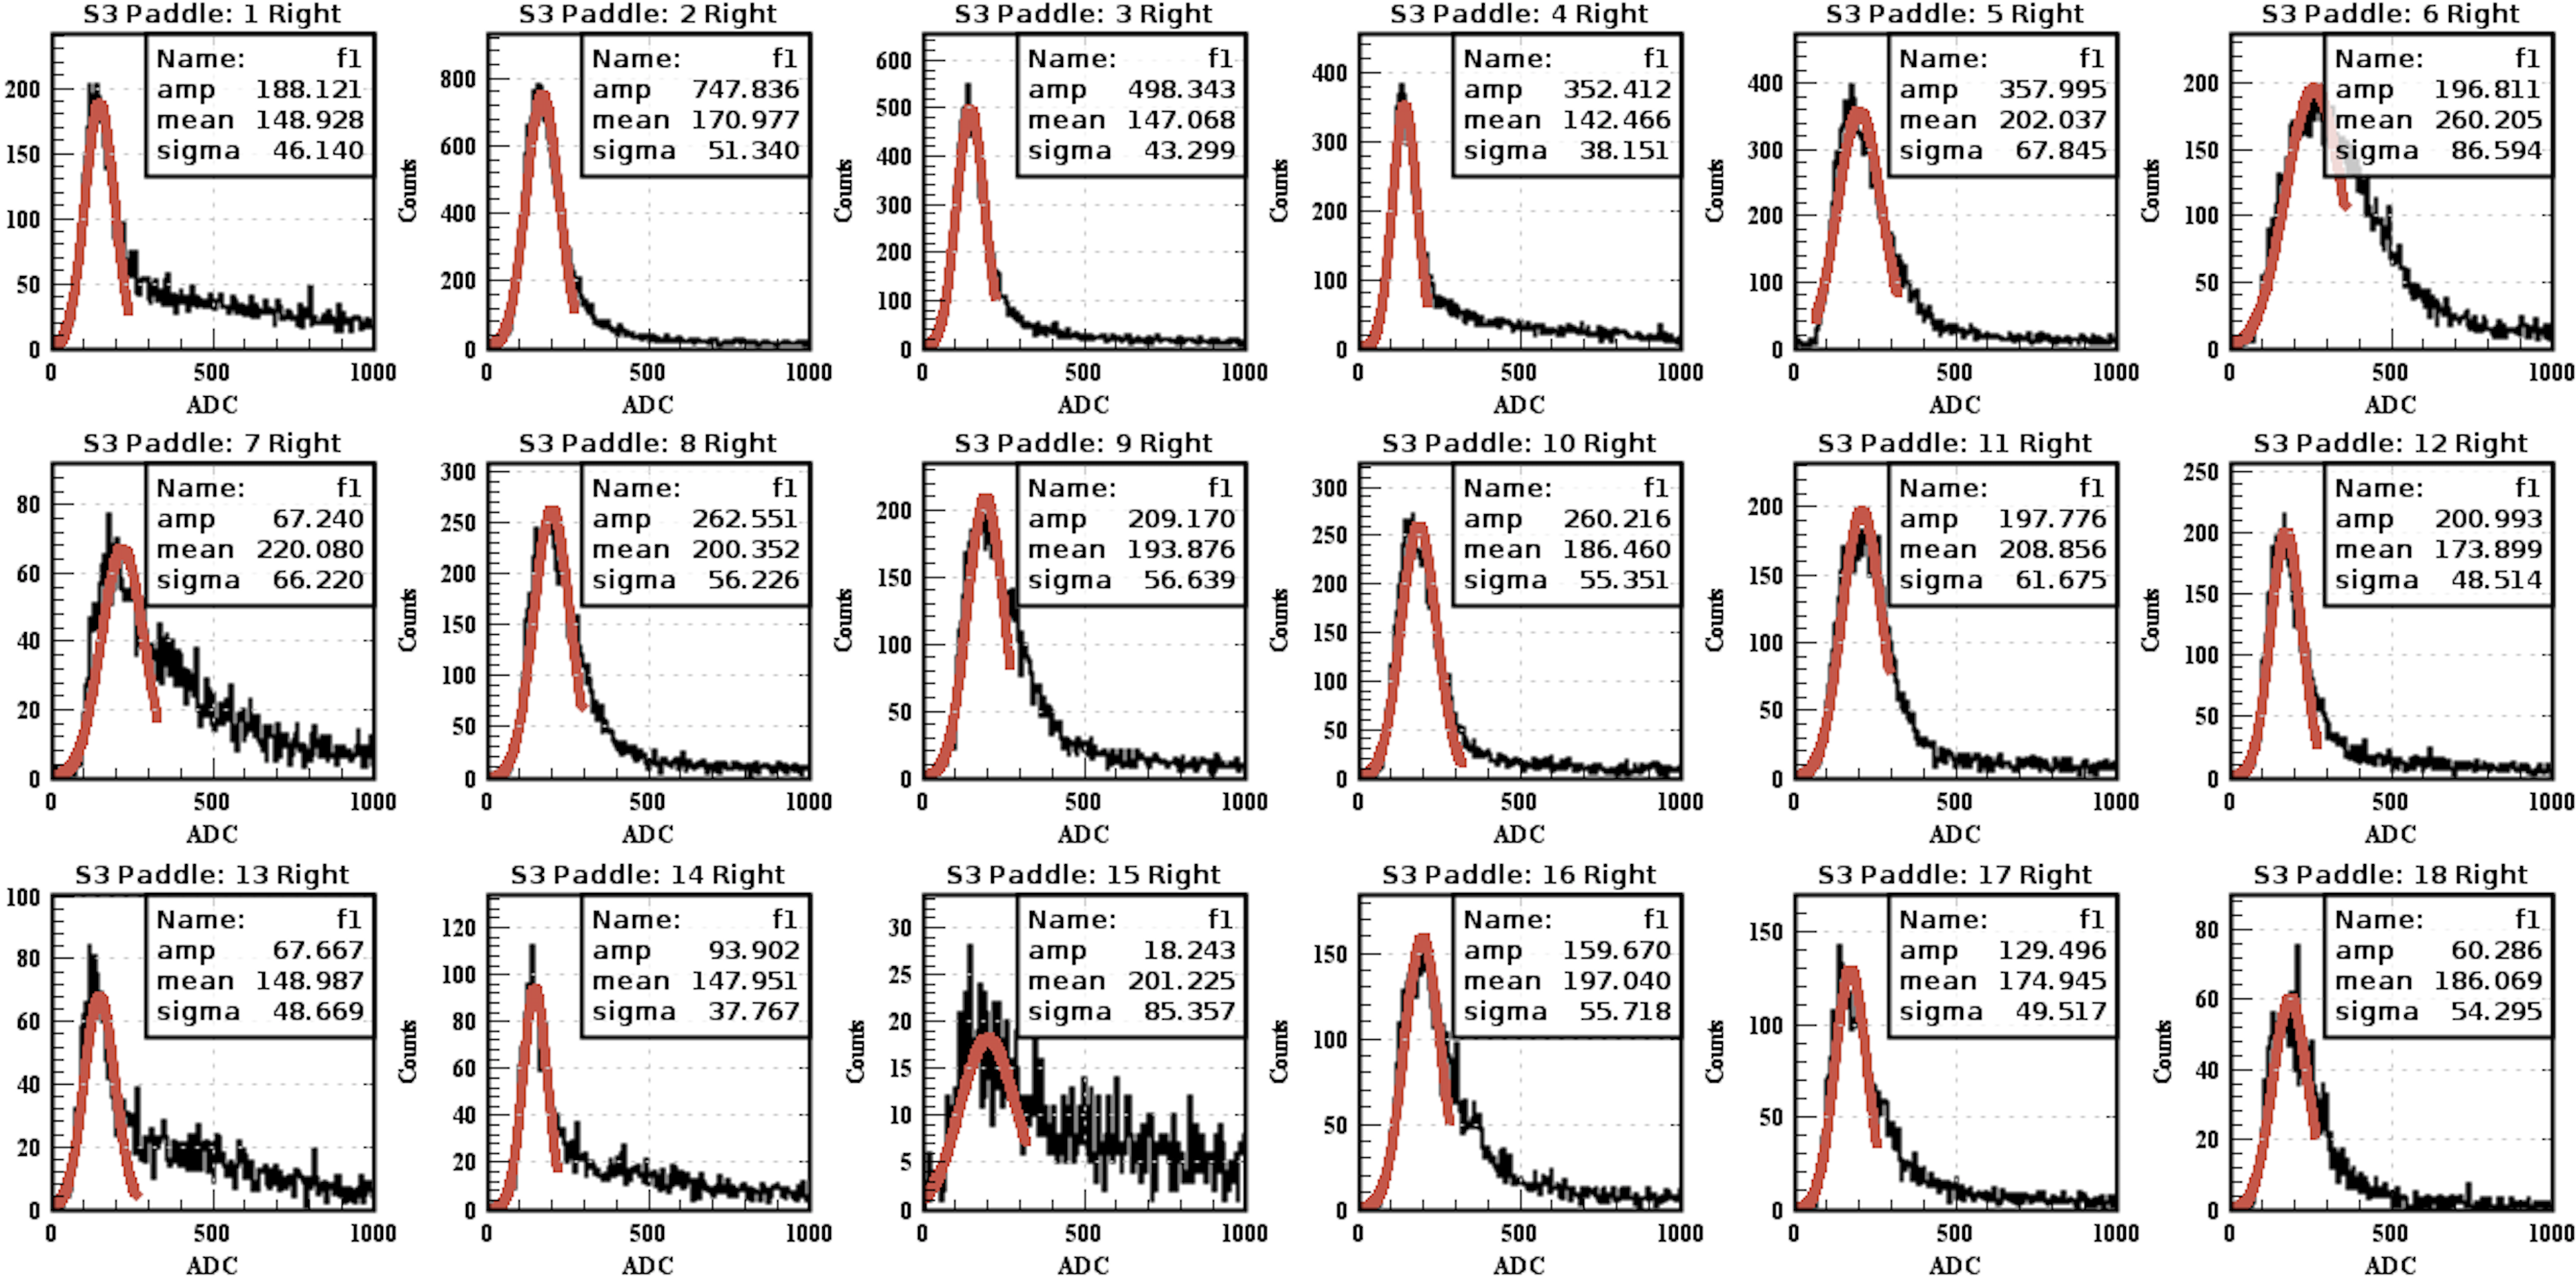
\includegraphics[width=0.98\columnwidth,keepaspectratio]{img/pimnphe.png}
	\caption{The number of photoelectrons as a function of $\theta$ and $\phi$ for 5 to 7 GeV pions. Top: positive pions. Bottom: negative pions}
	\label{fig:neutronMM}
\end{figure}



